\documentclass{article}
\usepackage{graphicx}
\usepackage{listings}
\usepackage[left=2cm, right=2cm]{geometry}
\title{Hand-in 1}
\author{Michael Iversen\\
Student ID: 201505099}

% Default fixed font does not support bold face
\DeclareFixedFont{\ttb}{T1}{txtt}{bx}{n}{10} % for bold
\DeclareFixedFont{\ttm}{T1}{txtt}{m}{n}{10}  % for normal

% Custom colors
\usepackage{color}
\definecolor{deepblue}{rgb}{0,0,0.5}
\definecolor{deepred}{rgb}{0.6,0,0}
\definecolor{deepgreen}{rgb}{0,0.5,0}

\usepackage{listings}
\usepackage{lipsum}
% Python style for highlighting
\newcommand\pythonstyle{\lstset{
		language=Python,
		basicstyle=\ttm,
		morekeywords={self},              % Add keywords here
		keywordstyle=\ttb\color{deepblue},
		emph={MyClass,__init__},          % Custom highlighting
		emphstyle=\ttb\color{deepred},    % Custom highlighting style
		stringstyle=\color{deepgreen},
		showstringspaces=false
}}

% Python environment
\lstnewenvironment{python}[1][]
{
	\pythonstyle
	\lstset{#1}
}
{}


\begin{document}
\maketitle
\section*{PART I: Logistic Regression}
	\subsection*{Code}
	\subsubsection*{Summary and results}
	Figure \ref{fig:logreg} shows the insample error as a function of epochs when applying the mini-batch gradient descent algorithm.
	As expected, the insample error slowly decreases as a function of epochs and eventually saturates.
	After $50$ epochs the insample accuracy is $\mathrm{Acc}_\mathrm{in} = 0.976$ and the test accuracy is $\mathrm{Acc}_\mathrm{test} = 0.956$.
	\begin{figure}
		\centering
		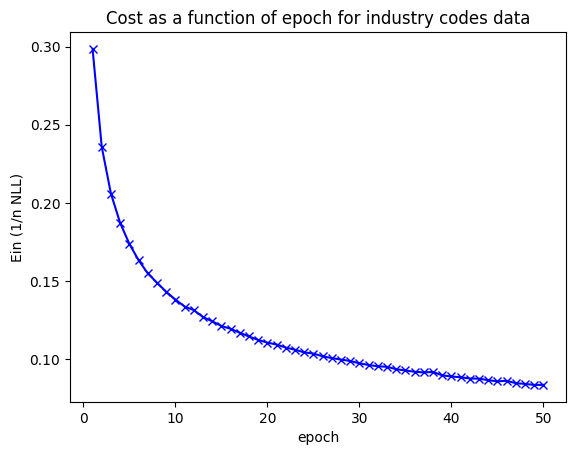
\includegraphics[width=0.5\textwidth]{logreg_text_cost_per_epoch.png}
		\caption{Insample error as a function of number of epochs for the logistic regression classifier}
		\label{fig:logreg}
	\end{figure}
	\subsubsection*{Actual code}
	The code below shows my implementation of the method ``cost\_grad''
	\begin{python}
def cost_grad(self, X, y, w):
	cost = np.mean(np.log(1 + np.exp(-X @ w * y)))
	grad = np.mean(-y * X.transpose() * logistic(-X @ w * y), axis=1)
	assert grad.shape == w.shape
	return cost, grad
	\end{python}
	Using this function, I implement the fitting method of the logistic regression classifier.
	\begin{python}
def fit(self, X, y, w=None, lr=0.1, batch_size=16, epochs=10):
	if w is None:
		w = np.zeros(X.shape[1])
	history = []
	for _ in range(epochs):
		permutation = np.random.permutation(np.arange(X.shape[0]))
		X_permuted = X[permutation, :]
		y_permuted = y[permutation]
		for idx_start in np.arange(0, X.shape[0], batch_size):
			idx_stop = idx_start + batch_size
			X_batch = X_permuted[idx_start:idx_stop, :]
			y_batch = y_permuted[idx_start:idx_stop]
			_, grad = self.cost_grad(X_batch, y_batch, w)
			w += -lr * grad
		cost, _ = self.cost_grad(X, y, w)
		history.append(cost)

	self.w = w
	self.history = history
	\end{python}
\subsection*{Theory}
	\subsubsection*{Time complexity}
	We investigate the running time to compute the cost and gradient in ``cost\_grad''.
	We start by studying the running time of computing the cost.
	Since the shape of $X$ is $n\times d$ and $w$ is $d \times 1$, the matrix product $X @ w$ has time complexity $O(nd)$.
	Multiplying the array $X @ w$ by $y$ is $O(n)$ and applying the operations $np.mean(np.log(1 + np.exp(\cdot)))$ to $X @ w * y$ is $O(n)$.
	Hence, computing the cost has time complexity $O(nd)$.

	Next, we investigate the time complexity of computing the gradient.
	The expression $y*X.transpose()$ involves broadcasting the array $y$ to size $d \times n$ and multiplying elementwise with $X$. 
	The time complexity of these computations is $O(nd)$.
	As discussed above, the time complexity of computing $X @ w * y$ is $O(nd)$.
	Applying the function $logistic(\cdot)$ to the array $X @ w * y$ is $O(n)$.
	Next, $logistic(-X @ w * y)$ is broadcast to size $d \times n$ and multiplied elementwise with $y * X.transpose()$ in $O(nd)$ time.
	Finally, the gradient is obtained by averaging the elements in each row which takes $O(nd)$ time.
	In total, the gradient is computed in $O(nd)$ time.
	
	We investigate the running time of the mini-batch gradient descent algorithm.
	The outermost for-loop executes the inside code $epochs$ times.
	Moving inside this for-loop, the permutation of $X$ and $y$ takes place in $O(n)$ time.
	The next for-loop executes the inside code $\lfloor n/batch\_size \rfloor$ times.
	Computing the cost and gradient of $X_{permuted}$, $y_{permuted}$ has complexity $O(d\cdot batch\_size)$.
	In total, the gradient descent algorithm has time complexity $O(epochs\cdot n d)$.
	
	The algorithm can be optimized by only computing the gradient (not the cost) in the innermost for-loop and only computing the cost (not the gradient) in the outermost for-loop. 
	However, this optimization does not change the time-complexity. 
	
	\subsubsection*{Sanity check}
	If the pixels in all images are randomly permuted (in the same way), I expect the classifier will perform as good as without the permutation.
	If the features are simply the rgb-values of each pixel, then our model does not use any information about the spatial location of each pixel. Hence, the performance is not affected by destroying the locality information by a permutation.
	If $\omega$ is an optimal model before the permutation, then $\omega' = \mathrm{P}(\omega)$ is an optimal model for the permuted data where $\mathrm{P}(\cdot)$ is the permutation of the pixels.
	
	\subsubsection*{Linearly separable data}
	When the data is linearly separable, the gradient descent algorithm finds weights so the insample error is very small $\mathrm{E_{in}}(w) = \frac{1}{n}\sum_{i=1}^n \mathrm{ln}(1 + e^{-y_i w^T x_i}) \approx 0$. Inspecting this expression, we see the optimal weights must cause the argument of the exponential function to be very large and negative for all data points, i.e. $y_i w^T x_i \gg 1$ for all $i$. These considerations yields the following interpretation of the optimal weights: for all data points $i$ with $y_i = 1$, the inner product between $w$ and the corresponding $x_i$ is very large and positive. Similarly, for all data points $i$ with $y_i = -1$, the inner product between $w$ and $x_i$ is very large and negative. One may think of $w$ ``pointing'' in the direction of all $x_i$ with $y_i=1$ and ``pointing'' in the opposite direction to all $x_i$ with $y_i = -1$.
\section*{PART II: Softmax}
\subsection*{Code}
\subsubsection*{Summary and results}
We test the code on two datasets: wine and written digits.
For the wine data set, the model reaches an insample accuracy of $\mathrm{Acc_{in}} = 1$ and test accuracy $\mathrm{Acc_{test}} = 0.978$. The build-in python implementation of softmax gives similar results.

When testing on the digit dataset, the model achieves an insample accuracy $\mathrm{Acc_{in}} = 0.918$ and test accuracy $\mathrm{Acc_{test}} = 0.920$.
I expect the softmax model to perform better on the digit data set if the features are transformed to exploit any information about locality present in the data set.

The insample error for the wine and digit data sets are illustrated in figure \ref{fig:softmax}.
\begin{figure}
	\centering
	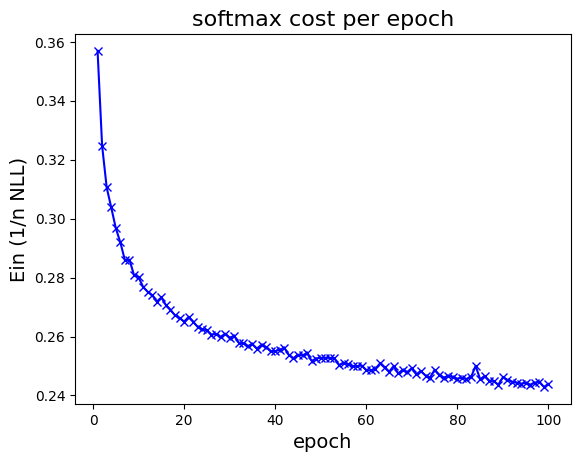
\includegraphics[width=0.49\textwidth]{softmax_cost_per_epoch}
	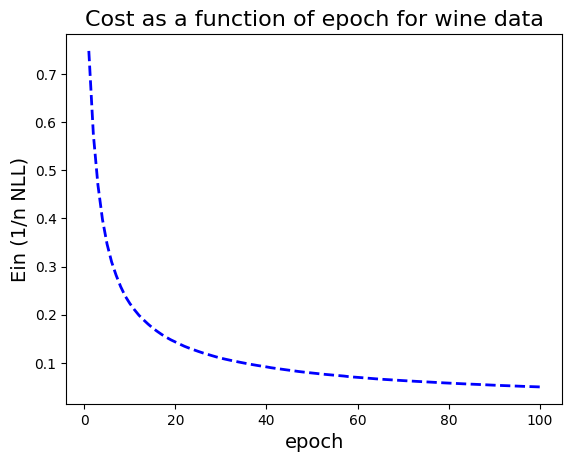
\includegraphics[width=0.49\textwidth]{softmax_wine_cost_per_epoch}
	\caption{The insample error as a function of the number of epochs for the digit (left panel) and wine (right panel) data sets. In both cases, the insample error decreases with increasing number of epochs as the algorithm finds a better and better model.}
	\label{fig:softmax}
\end{figure}

\begin{figure}
	\centering
	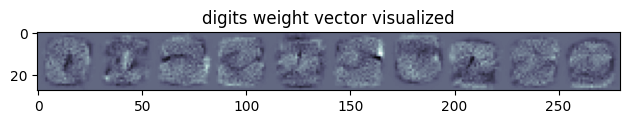
\includegraphics{softmax_weight_vector}
	\caption{The weight vector for the digit data set.}
\end{figure}
\subsubsection*{Actual code}
Below is my implementation of the function ``$cost\_grad$'' which computes the cost and gradient of the softmax model.
\begin{python}
def cost_grad(self, X, y, W):
	cost = np.nan
	grad = np.zeros(W.shape) * np.nan
	Yk = one_in_k_encoding(y, self.num_classes)
	n, d = X.shape
	cost = - np.mean(np.log(np.sum(Yk * softmax(X @ W), axis=1)))
	grad = - X.transpose() @ (Yk - softmax(X @ W)) / n
	return cost, grad
\end{python}
Using this function, I implement the mini-batch stochastic gradient descent algorithm.
\begin{python}
def fit(self, X, Y, W=None, lr=0.01, epochs=10, batch_size=16):
	if W is None:
		W = np.random.rand(X.shape[1], self.num_classes)
	history = []
	n, d = X.shape
	for epoch in range(epochs):
		permutation = np.random.permutation(np.arange(X.shape[0]))
		X_permuted = X[permutation, :]
		Y_permuted = Y[permutation]
		for batch in range(0, n, batch_size):
			x = X_permuted[batch:batch+batch_size, :]
			y = Y_permuted[batch:batch+batch_size]
			_, grad = self.cost_grad(x, y, W)
			W = W - lr * grad
		cost, _ = self.cost_grad(X, Y, W)
		history.append(cost)
	self.W = W
	self.history = history
\end{python}
\subsection*{Theory}
We investigate the time complexity of the ``$fit$'' function in the softmax model.
The analysis is similar to the discussion for the logistic regression model.
We start by inspecting the ``$cost\_grad$'' function.
The computation of both cost and gradient is dominated by the matrix product $X @ W$ which takes $O(ndK)$ for $n$ data points with $d$ weights and $K$ classes.
The outermost loop in the ``$fit$'' function executes the inside code $epochs$ times and the innermost loop executes $n/batch\_size$ times. Finally, the cost and gradient is calculated for $batch\_size$ data points with $d$ weights in $O(d \cdot batch\_size \cdot K)$ time.
The total time complexity is therefore $O(epochs \cdot n d K).$
	
\end{document}